\section{Les conditions initiales}
\begin{frame}
\frametitle{Approximations sur $T$ et $\Sigma$}
\begin{equation*}
	\dot{M} = 1\ 10^{-1 }\dot{M_{0}}
\end{equation*} 

	\begin{equation*}
	T = 1.4 \times 10^{4} \alpha^{- \frac{1}{5}} \left[ \frac{\dot{M}}{10^{16} \mathrm{g.s}^{-1}} \right]^{\frac{3}{10}} \left[ \frac{M}{M_\odot}\right]^{\frac{1}{4}} \left[ \frac{r}{10^{10}\mathrm{cm}}\right]^{- \frac{3}{4}} f^{\frac{3}{10}} \mathrm{K} 
\end{equation*}

\begin{equation*}
	\begin{aligned}
		\Sigma = 5.2 \alpha^{- \frac{4}{5}} \left[ \frac{\dot{M}}{10^{16} \mathrm{g.s}^{-1}} \right]^{\frac{7}{10}} \left[ \frac{M}{M_\odot}\right]^{\frac{1}{4}} \left[ \frac{r}{10^{10} \mathrm{cm}}\right]^{- \frac{3}{4}} f^{\frac{7}{10}} \mbox{K}  \\ 
	\text{avec } f = \left[ 1 - \left( \frac{r}{3 r_{s}}\right)^{- \frac{1}{2}}\right]
		\end{aligned}
\end{equation*}
\end{frame}

\begin{frame}
\frametitle{Approximations sur $T$ et $\Sigma$}
 \begin{figure}[ht]
   \begin{minipage}[c]{.46\linewidth}
      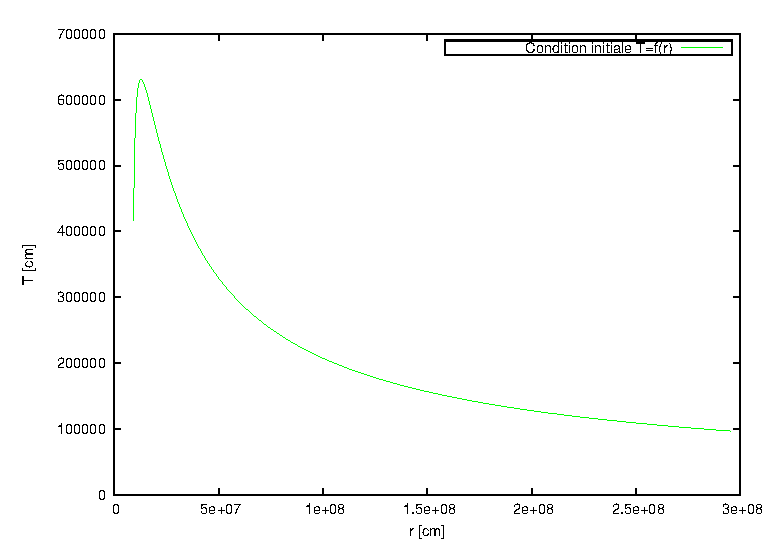
\includegraphics[scale=0.4]{ic_T.eps}
      \caption{Tracé de $T(r)$ à $t = 0$}
   \end{minipage} \hfill
   \begin{minipage}[c]{.46\linewidth}
      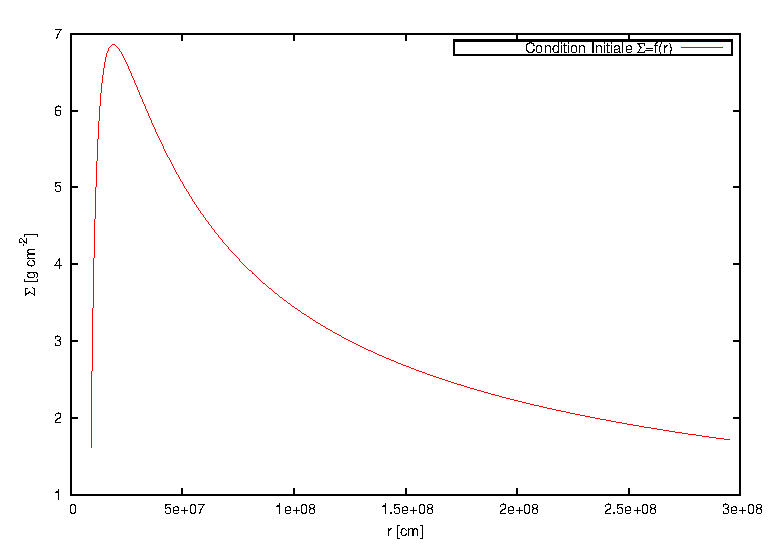
\includegraphics[scale=0.4]{ic_Sig.eps}
      \caption{Tracé de $\Sigma(r)$ à $t = 0$}
   \end{minipage}
\end{figure} 
\end{frame}

\begin{frame}
\frametitle{Approximation sur $H$}
	\begin{equation*}
	\frac{H}{r} = 1.7 \times 10^{-2}\alpha^{- \frac{1}{10}} \left[ \frac{\dot{M}}{10^{16} \mbox{g} \mbox{s}^{-1}} \right]^{\frac{3}{20}} \left[ \frac{M}{M_\odot}\right]^{- \frac{3}{8}} \left[ \frac{r}{10^{10} \mathrm{cm}}\right]^{\frac{1}{8}} f^{\frac{3}{5}}
\end{equation*}
\end{frame}

\begin{frame}
\frametitle{Approximation sur $H$}
	\begin{center}
		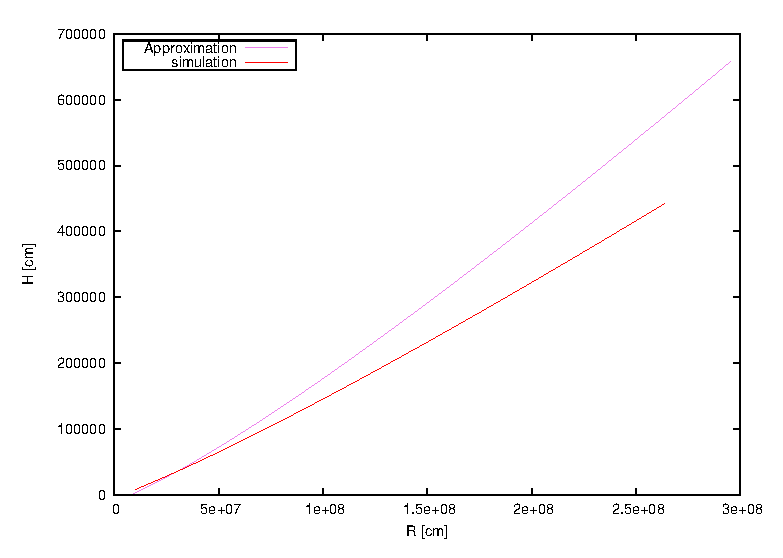
\includegraphics[scale=0.7]{ic_h.eps}
	\end{center}
\end{frame}

\begin{frame}
\frametitle{La vitesse angulaire $\Omega$}
	\begin{center}
		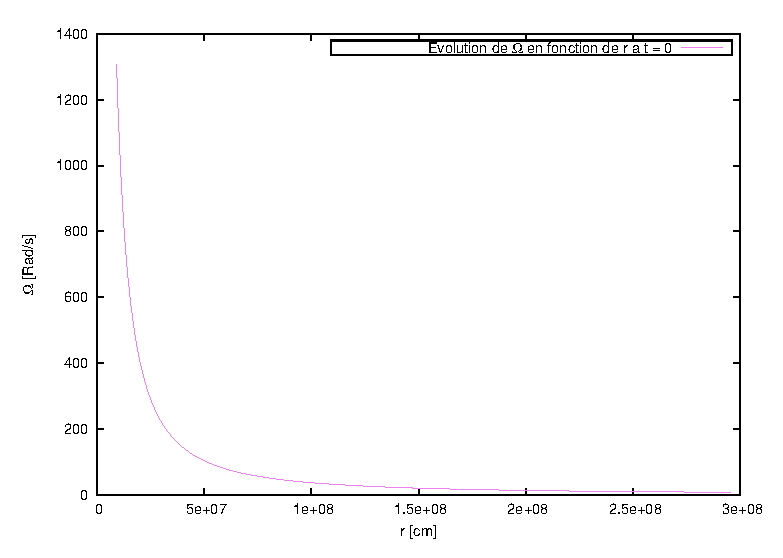
\includegraphics[scale=0.7]{Omega.eps}
	\end{center}
\end{frame}